\documentclass[twoside]{article}

\usepackage{lipsum}
\usepackage[none]{hyphenat} 

\usepackage[sc]{mathpazo} 
\usepackage[T1]{fontenc} 
\linespread{1.05}
\usepackage{microtype}

\usepackage[hmarginratio=1:1,top=32mm,columnsep=20pt]{geometry}
\usepackage{multicol} 
\usepackage[hang, small,labelfont=bf,up,textfont=it,up]{caption} 
\usepackage{booktabs} 
\usepackage{float} 
\usepackage{hyperref}
\usepackage{amsmath}

\usepackage{lettrine} 
\usepackage{paralist}

\usepackage{abstract} 
\renewcommand{\abstractnamefont}{\normalfont\bfseries}
\renewcommand{\abstracttextfont}{\normalfont\small\itshape} 

\usepackage{titlesec} 
\renewcommand\thesection{\Roman{section}} 
\renewcommand\thesubsection{\Roman{subsection}} 
\titleformat{\section}[block]{\large\scshape\centering}{\thesection.}{1em}{} 
\titleformat{\subsection}[block]{\large}{\thesubsection.}{1em}{}

\usepackage{fancyhdr} 
\pagestyle{fancy} 
\fancyhead{} 
\fancyfoot{}

\fancyhead[C]{ Estad\'istica $\bullet$ Equipo 5 $\bullet$ C-411}
\fancyfoot[RO,LE]{\thepage}

\title{\vspace{-0.5cm}\fontsize{20pt}{10pt}\selectfont\textbf{Proyecto Fase 2}}

\author{
\large
\textsc{\vspace{-2cm} Alejandro Campos, Darian Dominguez, Nelson Mendoza}\\[3.5cm]
\normalsize Facultad de Matem\'atica y Computaci\'on \\
\normalsize Universidad de la Habana \\
\normalsize 2021 \\[1cm]
\vspace{-5mm}
}
\date{}


\usepackage{graphicx}
\begin{document}

\maketitle

\thispagestyle{fancy} 

\begin{center}
\textbf{Resumen}
\end{center}
\noindent \textit{En la segunda fase del proyecto correspondiente a la asignatura de Estad\'istica se hace un estudio sobre los datos usados en la fase 1, en el que aplicaremos t\'ecnicas de regresi\'on lineal, ANOVA, y reducci\'on de dimensi\'on. Para ello se definen las variables pricipales que est\'an contenidas en el set de datos, sobre las que se realizaran las dos primeras t\'ecnicas. Adem\'as, se hace un an\'alisis de los supuestos de cada modelo a fin de investigar la validez de estos y se construyen gr\'aficas en cada t\'ecnica para analizar los resultados obtenidos de forma visual. El objetivo del proyecto es el an\'alisis de los datos usando las t\'ecnicas antes mencionadas. Con ayuda del software R y de R studio, se cre\'o la implementaci\'on que se puede encontrar en \texttt{code/fase\_2.R} de la cual nos auxiliaremos a lo largo de este informe.}\\[0.5cm]

\begin{multicols}{2}

\section{Introducci\'on}
La regresi\'on lineal o ajuste lineal es un modelo matem\'atico usado para aproximar la relaci\'on de dependencia entre una variable dependiente $Y$, y $m$ variables independientes $X_i$. El an\'alisis de la regresi\'on lineal consiste en encontrar la ecuaci\'on de la recta que mejor describe la relaci\'on entre las variables, siendo uno de los usos de esta ecuaci\'on hacer predicciones. El an\'alisis de la varianza (ANOVA) parte del concepto de regresi\'on lineal, cuya funcionalidad ampl\'ia. Es un procedimiento creado por Fisher en $1925$ para descomponer la variabilidad de un experimento en componentes independientes que puedan asignarse a causas distintas. As\'i, un an\'alisis de la varianza permite determinar si diferentes tratamientos muestran diferencias significativas en sus resultados o si, por el contrario, puede suponerse que sus medias poblacionales no difieren. Por lo que, a pesar de su nombre, es una t\'ecnica estad\'istica que permite la comparaci\'on de las medias de una caracter\'istica en varias poblaciones. Por \'ultimo, las t\'ecnicas de reducci\'on de dimensi\'on permiten, como su nombre lo indica, reducir el n\'umero de variables en una muestra o la cantidad de mediciones realizadas, agrupando en componentes/cl\'usters las variables/mediciones con caracter\'isticas similares. Para lograr esto se usa el an\'alisis de componentes principales y t\'ecnicas de clasificaci\'on como cl\'uster jer\'arquico, algoritmo k-means y \'arboles de clasificaci\'on. 

Todos los m\'etodos antes descritos se abordar\'an y ejemplificaran a lo largo de este informe, no sin antes explicar en qu\'e consiste el set de datos que se analizar\'a en cada secci\'on.\\\\




\section{Set de datos}
El set de datos que se analizar\'a a continuaci\'on es el conjunto de datos de Delft, utilizado para predecir el rendimiento hidrodin\'amico de los yates de vela a partir de las dimensiones y velocidad. Esta base de datos muestra el comportamiento de las siguientes variables:
\begin{enumerate}
\item Posici\'on longitudinal del centro de flotabilidad, adimensional.
\item Coeficiente prism\'atico, adimensional.
\item Relaci\'on longitud-desplazamiento, adimensional.
\item Relaci\'on haz-tiro, adimensional.
\item Relaci\'on longitud-haz, adimensional.
\item N\'umero de Froude, adimensional.
\item Resistencia residual por unidad de peso de desplazamiento, adimensional.\\
\end{enumerate}

\subsection{Variables principales}
De las variables anteriores se catalogan como principales, por su importancia, el coeficiente prism\'atico, el n\'umero de Froude y la resistencia residual. El coeficiente prism\'atico nos da una idea de c\'omo est\'a dise\~nado el barco para "penetrar" en el agua, es decir, la facilidad para que el barco se ponga a planear y aumente su velocidad. Indica, adem\'as, la relaci\'on entre el volumen sumergido y el volumen definido por su manga m\'axima. Dicho de otra manera, indica el cociente entre el volumen sumergido y el volumen de la pieza a partir de la cual se ha podido "tallar" el casco. Cuanto menor sea este coeficiente m\'as finos ser\'an la popa y proa y, por tanto, mejor afrontar\'an las olas. El n\'umero de Froude relaciona el efecto de las fuerzas de inercia y las fuerzas de gravedad que act\'uan sobre un fluido, estas fuerzas est\'an presentes en el accionar de las olas causadas por un barco al navegar, por ello, esta variable es de suma importancia para el rendimiento hidrodin\'amico de un buque. Con el n\'umero de Froude se puede predecir la resistencia al avance de los barcos, estimando la resistencia que estos presentan ante las olas, que depende de la resistencia de fricci\'on (debida a la superficie mojada del casco) y la resistencia residual (debida a la formaci\'on de olas). Finalmente, la resistencia residual por unidad de peso de desplazamiento es causada por la presi\'on que genera el casco al abrirse paso a trav\'es del agua, esta variable es de gran valor para los yates de vela en la etapa de dise\~no inicial,  para evaluar el rendimiento del buque y estimar la potencia propulsora requerida.\\





\section{Regresi\'on lineal}
Utilizaremos el m\'etodo backward para realizar un modelo de regresi\'on lineal que explique el comportamiento de la resistencia residual a partir del resto de las variables principales. Luego nuestro modelo comienza con todas las variables antes mencionadas, analicemos los resultados:\\

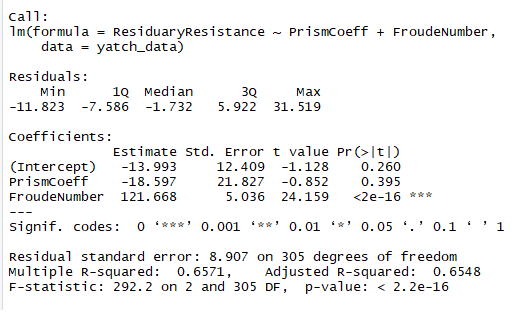
\includegraphics[scale = 0.5]{images/pic_01.png} \\

Podemos observar que la variable coeficiente prism\'atico (\textit{PrismCoeff}) ni el intercepto son significativos en el modelo, es decir, sus coeficientes no le aportan nada a este. \\
Si analizamos la matriz de correlaci\'on obtenemos: \\

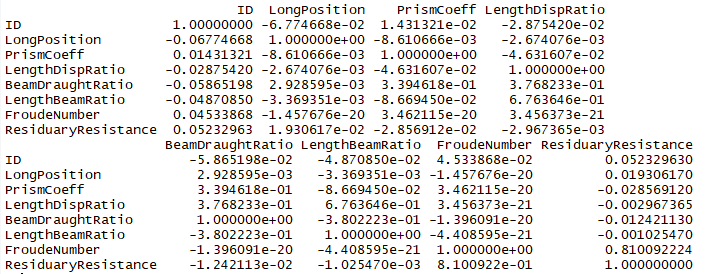
\includegraphics[scale = 0.4]{images/pic_02.png} \\

Al analizar la matriz es f\'acil darse cuenta de que las variables coeficiente prism\'atico y resistencia residual no est\'an correlacionadas, de hecho, ninguna de las variables est\'an correlacionadas entre s\'i, a excepci\'on del n\'umero de Froude y resistenia residual. Como, en el caso de este modelo en particular, la variable dependiente \textit{ResiduaryResistance} no est\'a correlacionada con la variable independente \textit{PrismCoeff}, debemos eliminarla. Por lo tanto tenemos un nuevo modelo sin la variable \textit{PrismCoeff} que, adem\'as hab\'iamos visto, no era significativa.\\

Luego llegamos a un modelo que tiene a \textit{ResiduaryResistance} como variable dependiente y a \textit{FroudeNumber} como variable independiente. Los resultados obtenidos con este modelo son los siguientes:\\

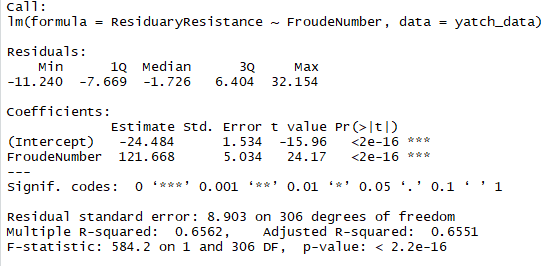
\includegraphics[scale = 0.4]{images/pic_03.png} \\

Ahora tenemos que Pr($>|t|$) de la variable independiente y del intercepto son menores que $0.05$. El p-value tambi\'en es menor que $0.05$. Por lo tanto, podemos proceder a hacer un an\'alisis de la presici\'on del modelo.\\
El modelo resultante es:\\

$\hat{ResiduaryResistance} = -24.484 + \\ 121.668 * FroudeNumber$\\

Se observa que el coeficiente del intercepto es mucho menor que el coeficiente del n\'umero de Froude, por lo tanto podemos decir que la mayor parte de la resistencia residual de los barcos est\'a explicada a partir del n\'umero de Froude. El coeficiente del n\'umero de Froude es significativo al $0\%$ y el del intercepto tambi\'en es significativo al $0\%$. Analizando los valores de estos coeficientes, se puede afirmar que por cada aumento unitario en el n\'umero de Froude debemos esperar que la resistencia residual aumente en $121.668$. \\

Pasando al an\'alisis de los residuos tenemos que el R-cuadrado ajustado es $0.66$, menor que $0.70$, por lo que podemos decir que  es un modelo bastante malo, no obstante, sigamos con el an\'alisis. El error est\'andar es $8.9$, no es tan peque\~no, no es lo ideal. El p-value del estad\'igrafo F, como se hab\'ia dicho, es menor que $0.05$, lo que quiere decir que existe al menos una variable significativamente diferente a cero en el modelo.\\

Veamos ahora si el modelo cumple los supuestos.\\
Recordemos que los supuestos son:
\begin{enumerate}
\item Existe una relaci\'on lineal entre las variables dependientes e independientes.
\item Los errores ($e_1,...,e_n$) son independientes.
\item El valor esperado del error aleatorio $e_i$ es cero ($E(e_i) = 0$)
\item La Varianza del error aleatorio es constante ($V(e_i) = \theta^2$). Homocedasticidad.
\item Los errores adem\'as de ser independientes son id\'enticamente distribuidos y siguen distribuci\'on normal con media cero y varianza constante ($e_i ~ N(0, \theta^2)$)
\item Las variables independientes del modelo no est\'an correlacionadas.
\end{enumerate}

Los supuestos $1$ y $6$ se cumplen en el modelo en cuesti\'on, pues el n\'umero de Froude esta correlacionado con la resistencia residual (ver matriz de correlaci\'on) y no hay m\'as variables independientes que el mismo n\'umero de Froude.\\
Realicemos un an\'alisis de los residuos para verificar si el resto de los supuestos se cumple:\\

Para analizar el cumplimiento del supuesto $3$ debemos verificar si la media de los errores es cero y la suma de los errores es cero. Con ayuda de los comandos de R, \textbf{mean} y \textbf{sum}, se llega a que, en efecto, este supuesto se cumple.\\

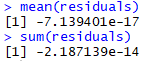
\includegraphics[scale = 0.7]{images/pic_04.png} \\

Para verificar el cumplimiento del supuesto $5$ debemos comprobar si los errores est\'an normalmente distribuidos. El histograma de residuos y el gr\'afico QQ-plot son formas de evaluar visualmente si los residuos siguen una distribuci\'on normal. Por tanto, buscamos que el histograma tenga forma de campana y en el QQ-plot que la mayor\'ia de los puntos de los residuos se encuentren sobre la recta o muy cercana a ella. Con ayuda de R construimos los gr\'aficos antes mencionados para este modelo:\\

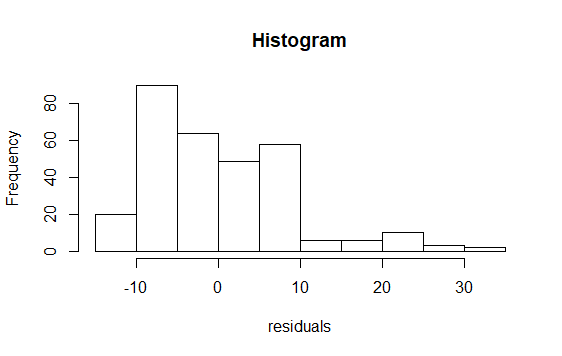
\includegraphics[scale = 0.4]{images/pic_05.png} \\
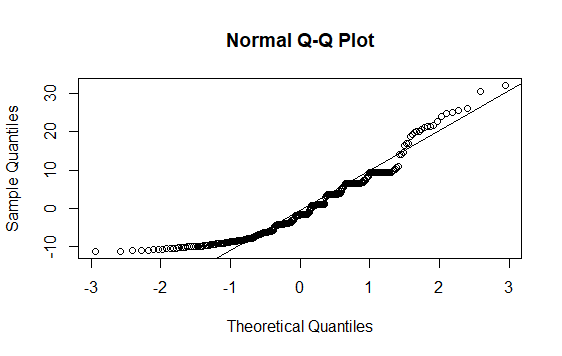
\includegraphics[scale=0.4]{images/pic_06.png} \\

Parece que los residuos no siguen una distribuci\'on normal, comprob\'emoslo con el test de Shapiro-Wilk, con ayuda de R.\\

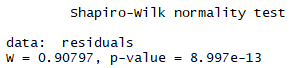
\includegraphics[scale = 0.6]{images/pic_07.png} \\

Como se observa, el p-valor del test de Shapiro-wilk es menor que $0.05$, luego se rechaza la hip\'otesis nula por lo que los errores no siguen una distribuci\'on normal. Ya hab\'iamos visto que este modelo era bastante malo, y ahora no cumple uno de los supuestos, por lo tanto ya podemos desecharlo. Sin embargo, analicemos el resto de los supuestos.\\

La prueba Durbin-Watson se usa para probar si los residuos son independientes. La hip\'otesis nula de esta prueba es que los errores son independientes.\\

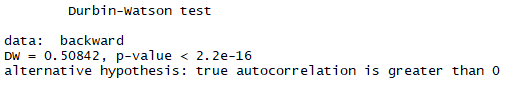
\includegraphics[scale=0.5]{images/pic_08.png} \\

Como el p-valor de esta prueba es menor que $0.05$ se rechaza la hip\'otesis nula, por lo que podemos afirmar que tampoco se cumple el supuesto $2$.\\

Para probar el supuesto $4$ de la Homocedasticidad podemos graficar los residuos como se muestra a continuaci\'on:\\

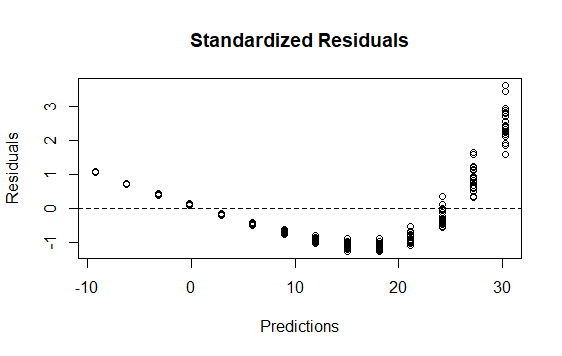
\includegraphics[scale = 0.4]{images/pic_09.png} \\
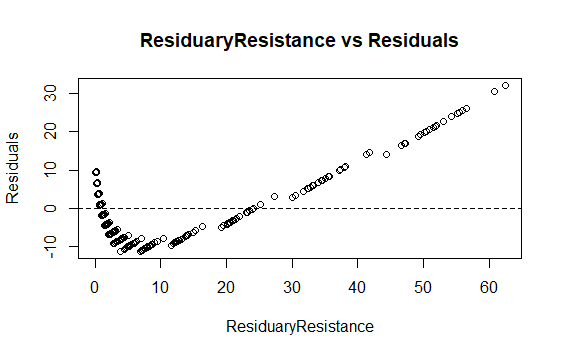
\includegraphics[scale=0.4]{images/pic_10.png} \\

Con estos gr\'aficos se comprueba que estos puntos no siguen una franja, por lo que es muy probable que este supuesto tampoco se cumpla. Utilicemos la prueba de Breusch-Pagan, que se utiliza para determinar la heterocedasticidad en un modelo de regresi\'on lineal, para verificar lo anterior.\\

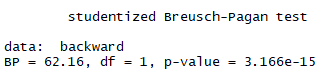
\includegraphics[scale=0.6]{images/pic_11.png} \\

Como el p-valor de esta prueba es menor que $0.05$ se rechaza la hip\'otesis nula por lo que  podemos afirmar que se cumple la heterocedasticidad. Por lo que el supuesto de Homocedasticidad no se cumple.\\\\

Se concluye que para estos datos no existe un modelo de regresi\'on lineal que se ajuste a ellos. 

No podemos dejar de mencionar que, dado el an\'alisis de la matriz de correlaci\'on realizado en esta secci\'on, no es posible utilizar otra combinaci\'on de variables para realizar otro modelo de regresi\'on, ya que las variables no tienen correlaci\'on entre s\'i, a excepci\'on de las que se analizaron. El \'unico modelo que se podr\'ia hacer con estos datos fue el que analizamos anteriormente, ya que el resto de combinaciones de modelos posibles no cumple, a priori, el supuesto $1$.

El an\'alisis de correlaci\'on tambi\'en se aborda de una forma mejor explicativa en la secci\'on V, subsecci\'on I del presente informe.\\\\




\section{ANOVA}
Realicemos un an\'alisis de ANOVA a fin de investigar si el n\'umero de Froude afecta la resistencia residual de los barcos veleros. Adem\'as, debemos considerar como factor secundario el coeficiente prism\'atico de estos. Es decir, tenemos la variable de estudio \textit{ResiduaryResistance}, y es claro que el n\'umero de Froude se puede ver como tratamiento y el coeficiente prism\'atico como bloque.

Luego el problema que acabamos de plantear responde al siguiente modelo estad\'istico de bloques: 
$$Y_{ij} = \mu + \alpha_i + \beta_j + e_{ij}$$ 
Donde $Y_{ij}$ es la medici\'on que corresponde al tratamiento $i$ y al bloque $j$, en este caso la resistencia residual de los barcos; $\mu$ es la media global poblacional; $\alpha_i$ es el efecto debido al tratamiento $i$, en este caso los distintos n\'umeros de Froude; $\beta_j$ es el efecto debido al bloque $j$, en este caso los distintos coeficientes prism\'aticos, y $e_{ij}$ es el error aleatorio atribuible a la medici\'on $Y_{ij}$.\\

La hip\'otesis que debemos formular es la siguiente:
\begin{align*}
H_0 &: \mu_1 = \mu_2 = ... = \mu_{14} = \mu \\
H_1 &: \mu_i \neq \mu_j \hspace{0.3cm} \text{para alg\'un} \hspace{0.3cm} i \neq j
\end{align*}

La cual se puede reescribir de forma equivalente como:
\begin{align*}
H_0 &: \alpha_1 = \alpha_2 = ... = \alpha_{14} = 0 \\
H_1 &: \alpha_i \neq 0 \hspace{0.3cm} \text{para alg\'un} \hspace{0.3cm} i 
\end{align*}

Primero deber\'iamos acomodar los datos para poder trabajar con ellos. Lo que buscamos es tenerlos de la siguiente forma:\\

\resizebox{6.5cm}{!}{
\begin{tabular}{| c | c | c |}
\hline
FroudeNumber & PrismCoeff & ResiduaryRes \\ \hline
f1 & p1 & r1 \\
f1 & p2 & r2 \\
f1 & p3 & r3 \\
\vdots & \vdots & \vdots \\
f1 & p10 & r10 \\
f2 & p1 & r11 \\
\vdots & \vdots & \vdots \\
f14 & p10 & r308 \\ \hline
\end{tabular}} \\\\

Como tenemos $14$ n\'umeros de Froude distintos y $10$ coeficientes prism\'aticos distintos, entonces ponemos en la primera columna secuencialmente $10$ veces el primer n\'umero de Froude, luego el segundo y as\'i sucesivamente, para poder listar en la segunda columna los valores de los coeficientes prism\'aticos en cada caso y, por \'ultimo, listar la resistencia residual de cada barco.\\

Luego necesitamos comparar las medias de los $14$ niveles del factor y las medias de los $10$ niveles del bloque. Para esto realizamos gr\'aficos de cajas con las medias de cada uno.\\

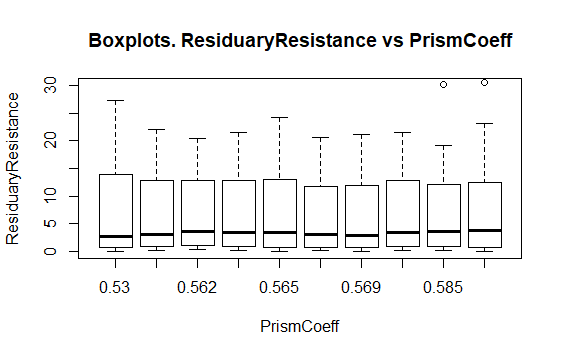
\includegraphics[scale = 0.4]{images/pic_12.png} \\
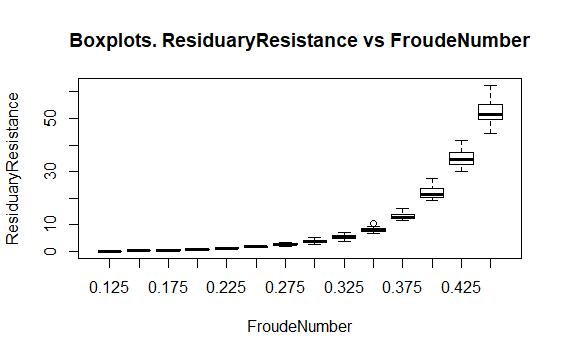
\includegraphics[scale=0.4]{images/pic_13.png} \\

Podemos observar que las medias de la resistencia residual de los coeficientes prism\'aticos son bastante cercanas, oscilando entre $2$ y $3$ aproximadamente, por lo que es posible que el coeficiente prism\'atico no tenga efecto sobre la resistencia residual de los veleros. 

Por otro lado, el gr\'afico de la resistencia residual y el n\'umero de Froude muestra mucha diferencia en las medias, podemos apreciar que empieza en valores muy cercanos a $0$ y, a medida que el n\'umero de Froude aumenta, obtenemos valores de resistencia residual promedio hasta de $50$. Por lo tanto, es muy probable que el n\'umero de Froude tenga efecto sobre la resistencia residual de los veleros.\\

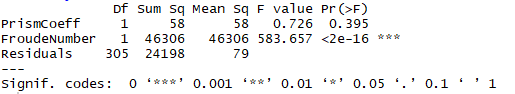
\includegraphics[scale = 0.4]{images/pic_14.png} \\

Notamos que en el caso del coeficiente prism\'atico el p-valor es mayor que $0.05$, luego no podemos rechazar $H_0$ por lo que se acepta que este no influye en la resistencia residual de los barcos.

En el caso del n\'umero de Froude, como el p-valor es menor que la significaci\'on prefijada $\alpha = 0.05$, entonces se rechaza $H_0$ y se acepta que al menos un par de n\'umeros de Froude tienen una resistencia promedio diferente, es decir, influyen sobre la resistencia residual de los barcos.\\

Verifiquemos si el modelo cumple los supuestos. Recordemos que estos son:
\begin{enumerate}
\item Los $e_{ij}$ siguen una distribuci\'on normal con media cero. 
\item Los $e_{ij}$ son independientes entre s\'i. 
\item Los residuos de cada tratamiento tienen la misma varianza $\theta^2$.\\
\end{enumerate}

Para verificar el cumplimiento del supuesto $1$ debemos comprobar si los errores est\'an normalmente distribuidos. El histograma de residuos y el gr\'afico QQ-plot son formas de evaluar visualmente si los residuos siguen una distribuci\'on normal. Por tanto, buscamos que el histograma tenga forma de campana y en el QQ-plot que la mayor\'ia de los puntos de los residuos se encuentren sobre la recta o muy cercana a ella. Con ayuda de R construimos los gr\'aficos antes mencionados para este modelo:\\

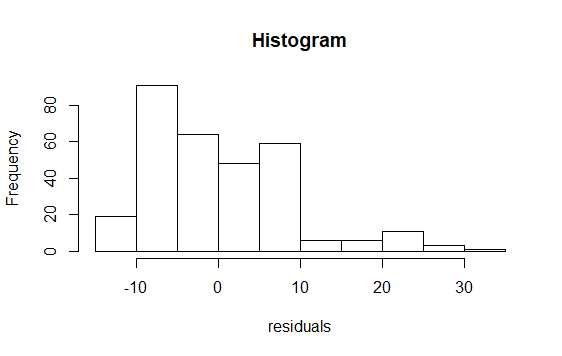
\includegraphics[scale = 0.4]{images/pic_15.png}
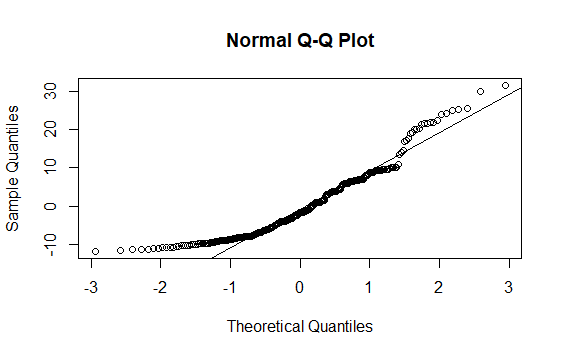
\includegraphics[scale=0.4]{images/pic_16.png} \\

Parece que los residuos no siguen una distribuci\'on normal, utilizaremos el test de Shapiro-Wilk, con ayuda de R, para comprobarlo.\\

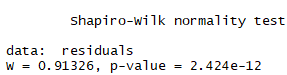
\includegraphics[scale = 0.6]{images/pic_17.png} \\

Como se observa, el p-valor del test de Shapiro-wilk es menor que $0.05$, luego se rechaza la hip\'otesis nula por lo que los errores no siguen una distribuci\'on normal. Podemos desechar este modelo, no obstante, analicemos el resto de los supuestos.\\

La prueba Durbin-Watson se usa para probar si los residuos son independientes. La hip\'otesis nula de esta prueba es que los errores son independientes.\\

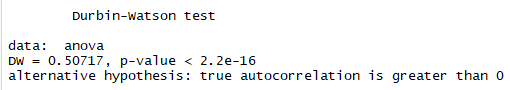
\includegraphics[scale = 0.5]{images/pic_18.png} \\

Como el p-valor de esta prueba es menor que $0.05$ se rechaza la hip\'otesis nula, por lo que podemos afirmar que tampoco se cumple el supuesto $2$.\\

Por \'ultimo, para probar el supuesto $3$ de la Homocedasticidad podemos graficar los residuos como se muestra a continuaci\'on:\\

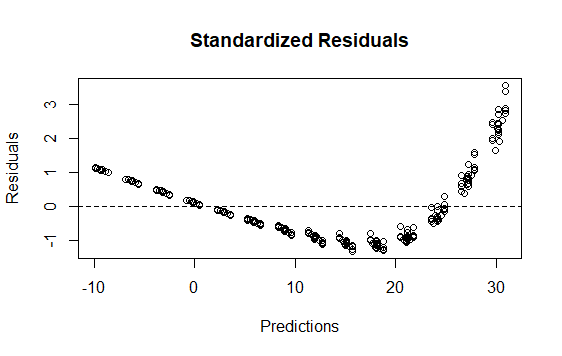
\includegraphics[scale = 0.4]{images/pic_19.png} \\

Los puntos no forman una franja, parece ser no que tienen varianza constante. Utilicemos la prueba de Bartlett para confirmarlo.\\

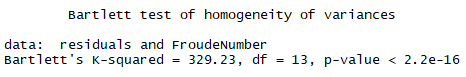
\includegraphics[scale = 0.5]{images/pic_20.png} \\

Como el p-valor de esta prueba es menor que $0.05$ se rechaza la hip\'otesis nula por lo que el supuesto de Homocedasticidad no se cumple.\\\\

De forma an\'aloga a como se desarroll\'o en esta secci\'on, se realizaron varios an\'alisis de ANOVA considerando otras variables, pero por desgracia ninguno result\'o v\'alido. Solo se refleja en este informe el realizado con las variables principales definidas previamente, cuyo modelo analizamos en esta secci\'on.\\\\




\section{Reducci\'on de dimensi\'on}
Realizaremos en esta secci\'on varias t\'ecnicas de reducci\'on de dimensi\'on a nuestro set de datos, ya sea en cuanto la cantidad de variables como en el tama\~no de la muestra.\\


\subsection{An\'alisis de componentes principales}
El objetivo del ACP es reducir dimensi\'on agrupando variables en componentes principales incorrelacionadas entre s\'i. En el caso de nuestro set de datos, como ya vimos en la secci\'on II, tenemos 7 variables.

Lo primero que debemos estudiar es la correlaci\'on de nuestra muestra. Para ello primero graficamos los datos para ver si existe alg\'un tipo de correlaci\'on entre ellos.\\

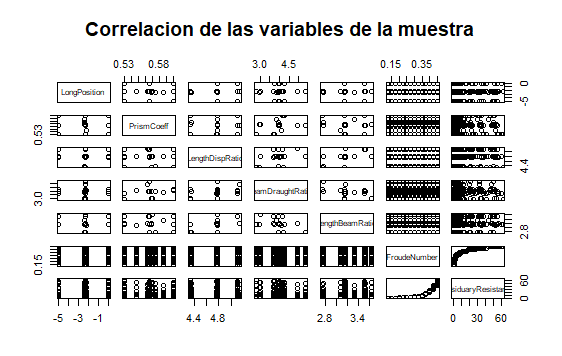
\includegraphics[scale = 0.4]{images/pic_21.png} \\

Son demasiadas variables para analizar de forma visual. Debemos acudir entonces a la matriz de correlaci\'on, analizada en la secci\'on III, pero esta vez trabajaremos con esta matriz en forma gr\'afica.\\

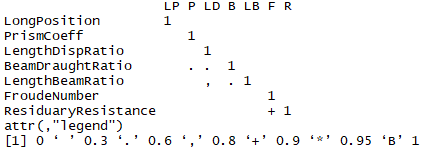
\includegraphics[scale = 0.5]{images/pic_22.png} \\

Como se puede apreciar no es una matriz altamente correlacionada, y solo tiene una marcada correlaci\'on el n\'umero de Froude y la resistencia residual, denotado con el s\'imbolo de $+$. 

En este caso ya las variables son independientes, por lo que este an\'alisis solo servir\'ia para reducir dimensi\'on. As\'i que podemos proseguir a realizar el ACP, obteniendo los siguientes resultados:\\

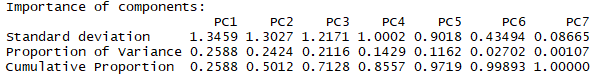
\includegraphics[scale = 0.4]{images/pic_23.png} \\

Ahora debemos escoger nuestras componentes principales. Seg\'un el criterio de Kaiser nos quedar\'iamos con las cuatro primeras componentes, explicando estas el $86\%$ de la muestra. Pero no hacemos mucho reduciendo a cuatro componentes dado que tenemos 7 variables. Por tanto, como el valor propio de la cuarta componente est\'a a solo $0.0002$ por encima de $1$, y como las tres primeras componentes explican el $71\%$ de la muestra, entonces nos quedaremos con PC1, PC2 y PC3.

Podemos, adem\'as, ver las componentes de forma visual para ratificar nuestra decisi\'on. Si graficamos estas componentes obtenemos:\\

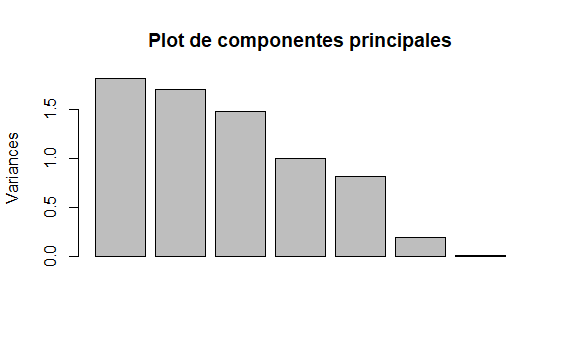
\includegraphics[scale = 0.4]{images/pic_24.png} \\

Se puede observar que a partir de la cuarta componente hay una ca\'ida m\'as pronunciada y que con las tres primeras se explica una buena parte, ser\'ia un $71\%$, que si bien no es lo ideal, no est\'a mal.

Ahora analizamos la matriz de valores propios y as\'i sabremos qu\'e variable es importante para cada componente y en qu\'e medida.\\

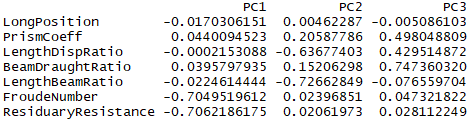
\includegraphics[scale = 0.5]{images/pic_25.png} \\

Comencemos por la primera componente. Tomamos el mayor valor propio modularmente, $0.71$, y lo dividimos entre $2$, dando como resultado $0.36$. Luego todo valor propio cuyo m\'odulo est\'e por encima de $0.36$ en la columna de la PC1 nos dar\'a las variables que conforman esta componente. Por tanto, la interpretaci\'on ser\'ia que la primera componente est\'a caracterizada por barcos que tienen bajo n\'umero de Froude y baja resistencia residual, o sea, son yates que pueden ignorar casi por completo la resistencia por olas en su navegaci\'on. 

Siguiendo el mismo an\'alisis para la segunda componente tenemos que el mayor valor abosluto de valores propios es $0.73$, dividido entre 2 ser\'ia $0.37$, por tanto, en esta componente los barcos tienen baja relaci\'on longitud - desplazamiento y tambi\'en una baja relaci\'on longitud - haz, o sea, son yates que est\'an hechos para "planear en el agua", es decir, alcanzan una gran velocidad. 

En la tercera componente tenemos que el mayor valor propio modular es $0.75$, dividido entre 2 es $0.38$, entonces esta componente est\'a representada por veleros que tienen un alto coeficiente prism\'atico, una elevada relaci\'on longitud - desplazamiento y una elevada relaci\'on haz - tiro, por lo que son yates veleros que no est\'an dise\~nados para alcanzar una velocidad muy alta.\\

Por \'ultimo, podemos ver un biplot del ACP.\\

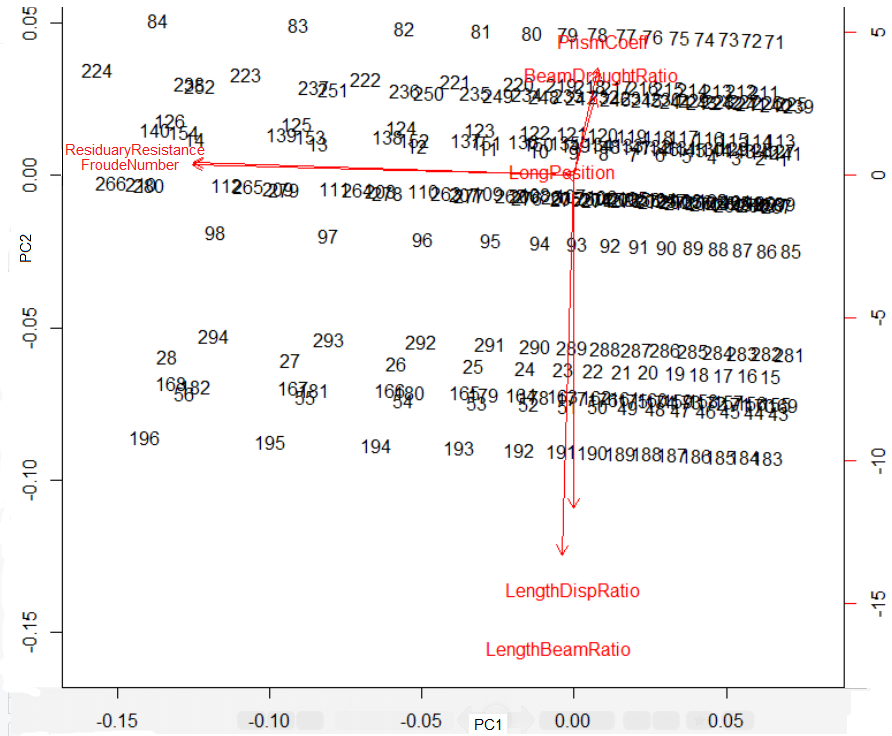
\includegraphics[scale = 0.3]{images/pic_26.png} \\

Primero se puede ver que las variables que representan la PC1 son n\'umero de Froude y resistencia residual de forma negativa pues tienen un \'angulo obtuso. La PC2 tiene como variables a la relaci\'on longitud desplazamiento y la relaci\'on longitud - haz de forma negativa. Mientras m\'as larga sea la recta que define a una variable m\'as representada est\'a la variable en la componente y m\'as importante ser\'a dentro de la misma. Tambi\'en podemos observar algunos yates que est\'an cerca de cada componente.\\\\


\subsection{Cl\'uster jer\'arquico}
Entre las t\'ecnicas para la reducci\'on de dimensi\'on se encuentran las t\'ecnicas de clasificaci\'on, que tienen como objetivo agrupar individuos de grandes poblaciones para reducir la dimensi\'on de la muestra. 

A partir de esta subsecci\'on nos centraremos en aplicar t\'ecnicas para reducir el tama\~no de la muestra.

El primer paso, independientemente del procedimiento a seguir, ser\'a estandarizar los datos para evitar errores en la clasificaci\'on por cuestiones de variabilidad en las unidades de medidas. Para esto tipificaremos cada una de las 7 variables. Obteniendo
$Z_i = \frac{X_i - \mu_i}{\sigma_i}$.

Para estandarizar usamos la funci\'on de R \textbf{scale}, y como se observa a continuaci\'on los datos estandarizados tienen el mismo comportamiento que los que no fueron estandarizados, la diferencia est\'a en la escala de las mediciones que es similar.\\

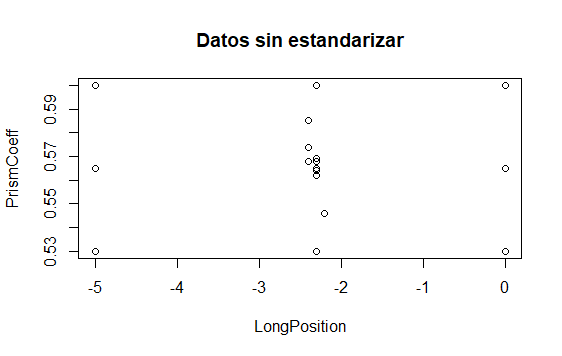
\includegraphics[scale = 0.4]{images/pic_27.png} \\
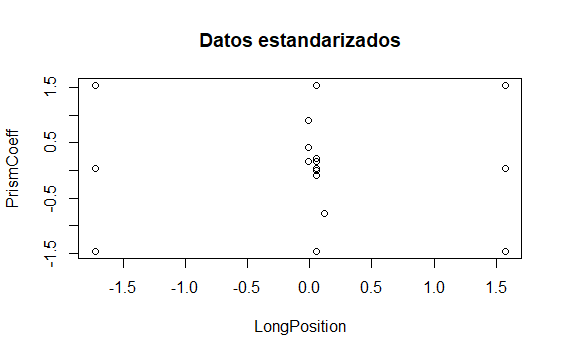
\includegraphics[scale = 0.4]{images/pic_28.png} \\

Una vez escaladas las mediciones construimos la matriz de distancias que ser\'a sim\'etrica, para la cual utilizamos la distancia euclidiana. Luego realizamos un cl\'uster jer\'arquico con el m\'etodo de ajuste completo y la matriz de distancias. Si graficamos el ajuste obtendremos el Dendograma del cl\'uster jer\'arquico.\\

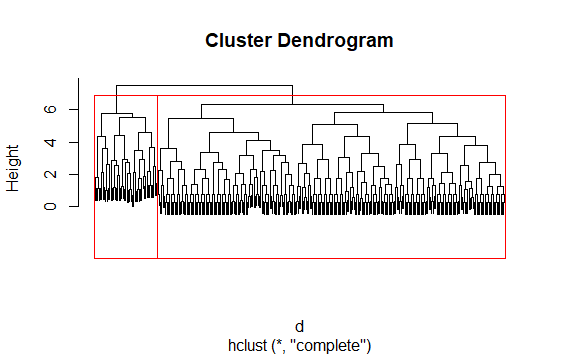
\includegraphics[scale = 0.5]{images/pic_29.png} \\

A partir de este gr\'afico podemos determinar la cantidad de cl\'usters haciendo cortes horizontales a alturas determinadas. Por ejemplo, si cortamos a altura poco mayor que $6$, obtendremos dos cl\'usters, como pudimos observar en la figura, uno que contiene a un peque\~no grupo de yates y otro que contiene al resto. Pero no tiene sentido, a pesar de que un peque\~no grupo de veleros se comporte de manera distinta, analizar el resto de los barcos como uno solo, pues si bajamos la altura vemos que ese gran cl\'uster se divide en cl\'usters m\'as peque\~nos. Tampoco tendr\'ia sentido realizar un an\'alisis por debajo de la altura $4$ pues tendr\'iamos muchos cl\'usters de elementos muy parecidos. En este caso decidimos quedarnos con $4$ cl\'usters como se muestra a continuaci\'on.\\

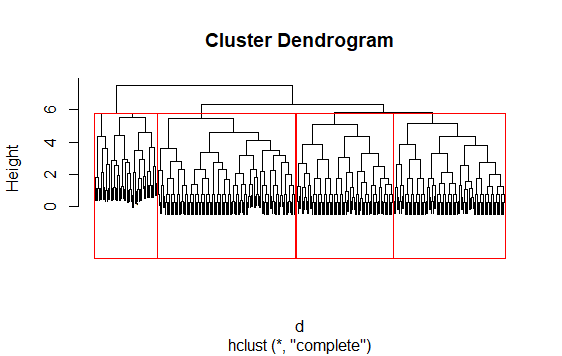
\includegraphics[scale = 0.5]{images/pic_30.png} \\

Por desgracia los cl\'usters son demasiado grandes y no quedan legibles los barcos que forman parte de cada uno. No obstante, podemos hacernos una idea de ese peque\~no grupo de yates que se comporta de manera distinta. Si analizamos los datos, nos percatamos de que existen algunos veleros que tienen una resistencia residual bastante alta y una posici\'on longitudinal muy baja, motivo por el cual se comportan de forma distinta a la mayor\'ia de los yates. Estos barcos podr\'ian formar parte del primer cl\'uster.

Todas las t\'ecnicas de cl\'uster jer\'arquico no dan los mismos resultados, veamos que sucede si en vez de utilizar un ajuste completo ajustamos por las medias. En este caso los ajustes son las medidas de asociaci\'on entre las variables.\\

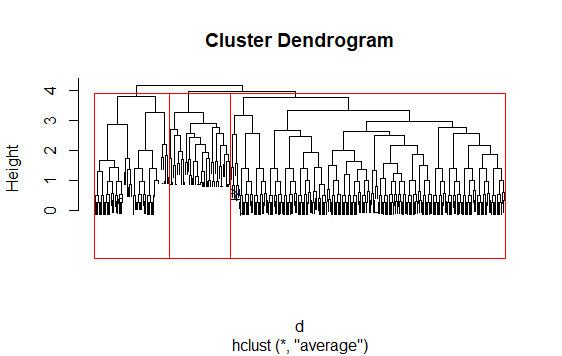
\includegraphics[scale=0.5]{images/pic_31.png} \\

Podemos notar que, a diferencia del ajuste completo, si hacemos un corte muy elevado obtenemos tres cl\'usters de yates que se comportan de manera diferente, dos relativamente peque\~nos y uno que contiene a la mayor\'ia de los yates.\\\\




\subsection{K-means}
Habiendo realizado la clasificaci\'on por el m\'etodo jer\'arquico, utilicemos ahora el algoritmo k-means. El problema m\'as grande al aplicar este algoritmo es que necesitamos tener una idea de cu\'antos cl\'usters tendremos, en este caso partiremos del n\'umero de cl\'usters encontrados en el algoritmo anterior. Es decir, comenzaremos con $4$ cl\'usters.\\

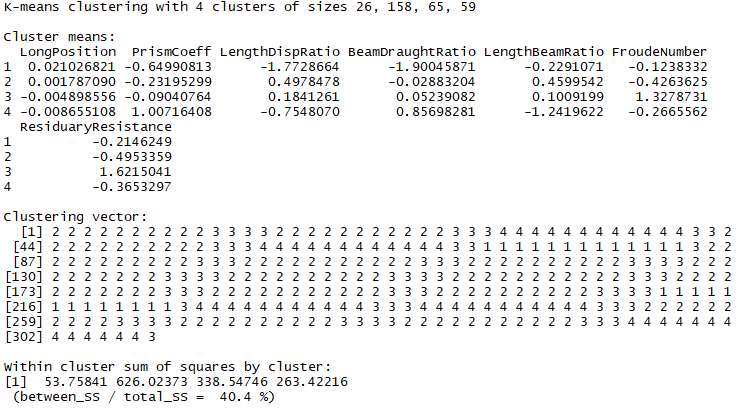
\includegraphics[scale=0.3]{images/pic_32.png} \\

Al aplicar la funci\'on k-means y comprobar su resultado obtenemos un vector de cl\'usters que nos dice en qu\'e cl\'uster est\'a cada barco y cu\'antos elementos hay. En este caso tenemos $4$ cl\'usters con $26$, $158$, $65$ y $69$ barcos respectivamente. Notemos que sigue habiendo un cl\'uster con un peque\~no grupo de barcos que se comportan de forma distinta.

Tambi\'en tenemos las medias de los elementos de cada variable por cada cl\'uster y, una de las informaciones m\'as importantes que podemos obtener, es la medida de similitud entre los elementos de cada cl\'uster, en este caso ser\'ia un $40.4\%$, que no es bueno. Debemos, al menos, duplicar la cantidad de cl\'usters para elevar un poco ese porcentaje.

Repetimos el algoritmo esta vez con $8$ cl\'usters.\\

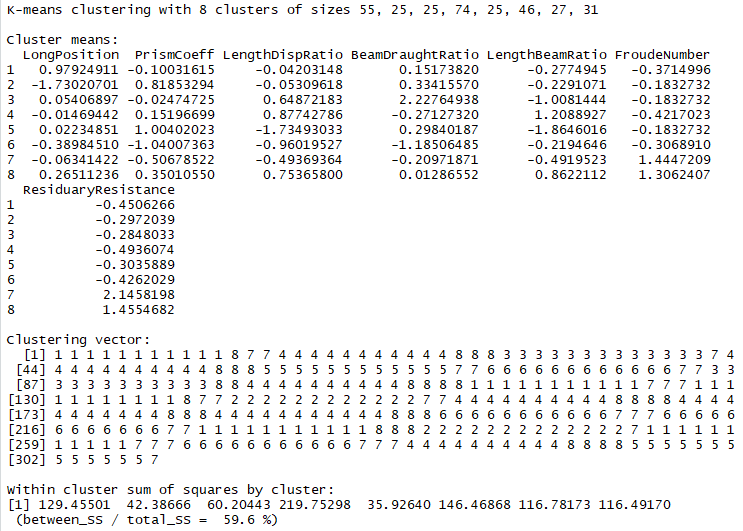
\includegraphics[scale=0.3]{images/pic_33.png} \\

Esta vez obtuvimos un porcentaje del $60\%$ que no est\'a mal. Y tampoco es exagerada la cantidad de cl\'usters, teniendo en cuenta que estamos trabajando una muestra de cardinalidad igual a $308$.

Si graficamos el resultado de k-means obtendremos una matriz de gr\'aficos.\\

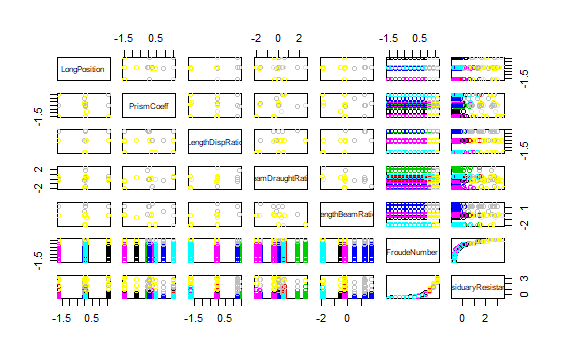
\includegraphics[scale=0.5]{images/pic_34.png} \\

La cual resulta imposible de analizar, por lo que si queremos analizar las relaciones de forma visual entre variables debemos analizarlas dos a dos, por ejemplo, resistencia residual y coeficiente prism\'atico.\\

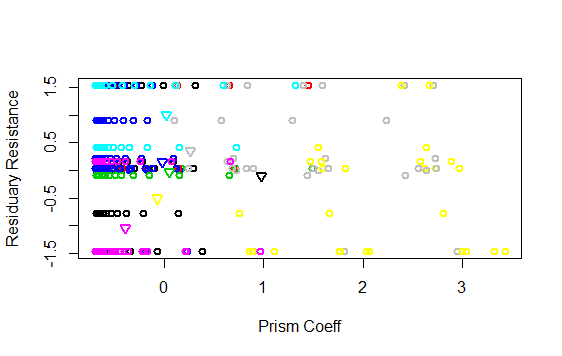
\includegraphics[scale=0.5]{images/pic_35.png} \\

Podemos observar los distintos cl\'usters representados con colores distintos. Adem\'as se han representado los centros de cada uno con tri\'angulos.


\subsection{\'Arboles de clasificaci\'on}
En esta secci\'on construiremos un \'arbol de clasificaci\'on para nuestros datos. Los \'arboles de clasificaci\'on son un m\'etodo usado en distintas disciplinas como modelo de predicci\'on. Estos son similares a diagramas de flujo, en los que llegamos a puntos en los que se toman decisiones de acuerdo a una regla.

Hay distintas maneras de obtener estos \'arboles, la que usaremos en esta ocasi\'on es conocida como CART: Classification And Regression Trees. Esta es una t\'ecnica de aprendizaje supervisado. Tenemos una variable objetivo (dependiente) y nuestra meta es obtener una funci\'on que nos permita predecir, a partir de variables predictoras (independientes), el valor de la variable objetivo para casos desconocidos.

En este caso la idea es ser capaz de predecir la resistencia residual de un yate velero basado en el resto de las variables que se brindan. La implementaci\'on particular de CART que usaremos es conocida como Recursive Partitioning and Regression Trees o RPART. De ah\'i el nombre del paquete que utilizaremos. De manera general, lo que hace este algoritmo es encontrar la variable independiente que mejor separa nuestros datos en grupos, que corresponden con las categor\'ias de la variable objetivo. Esta mejor separaci\'on es expresada con una regla. A cada regla corresponde un nodo.

Lo primero es escoger los conjuntos de entrenamiento y de prueba que ser\'an conjuntos disjuntos, en este caso se toman dos tercios de la poblaci\'on para el conjunto de entrenamiento y el tercio restante servir\'a para probar el \'arbol y calcular el error de clasificaci\'on.

Usamos la funci\'on de R \textbf{rpart} de la librer\'ia \textit{rpart} para entrenar nuestro modelo y obtenemos el siguiente resultado.\\

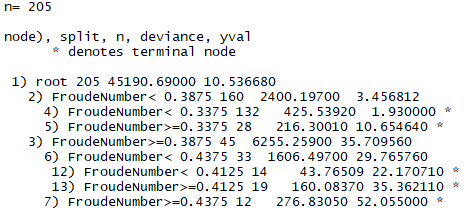
\includegraphics[scale=0.5]{images/pic_36.png} \\

Lo anterior muestra el esquema de nuestro \'arbol de clasificaci\'on. Cada inciso nos indica un nodo y la regla de clasificaci\'on que le corresponde. Siguiendo estos nodos, podemos llegar a las hojas del \'arbol, que corresponde a la clasificaci\'on de nuestros datos. Todo lo anterior resulta mucho m\'as claro si lo visualizamos, as\'i que creamos la siguiente gr\'afica usando nuestro modelo.\\

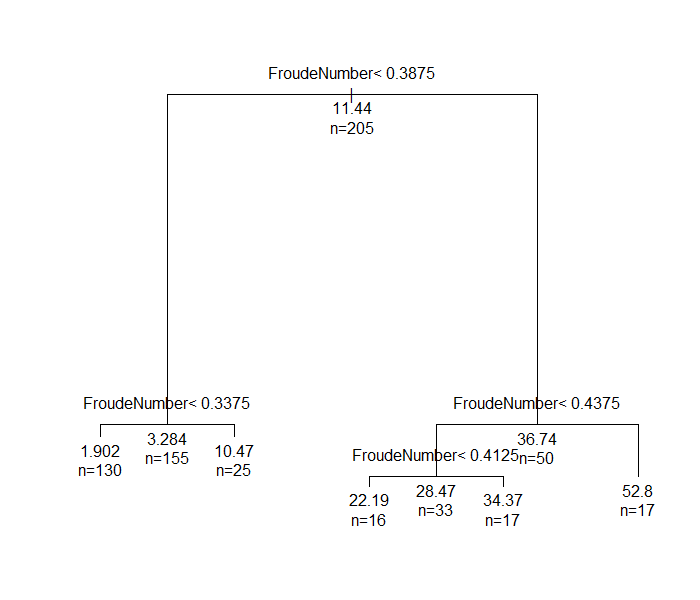
\includegraphics[scale=0.5]{images/pic_37.png}\\

En este gr\'afico, cada una de las intersecciones representa un nodo de nuestro \'arbol, con su regla de clasificaci\'on. Tengamos en cuenta que si bajamos por su rama izquierda estamos asumiendo que la regla se cumple. De esta forma si tenemos un velero con un n\'umero de Froude menor que $0.34$ nuestro \'arbol predice que la resistencia residual de este ser\'a de $1.9$. Si el n\'umero de Froude es menor que $0.38$ y mayor que $0.34$ ($0.34 \leq FroudeNumber < 0.39$) la resistencia residual del barco ser\'a de $10.47$. Por otro lado, si el n\'umero de Froude es menor que $0.41$ tendr\'iamos una resistencia residual de $22.19$. Si $0.41 \leq FroudeNumber < 0.44$ entonces la resistencia residual ser\'ia igual a $34.37$. Por \'ultimo, si $FroudeNumber \geq 0.44$ implica que la resistencia residual del velero tendr\'ia un valor de $52.8$.

Posteriormente podaremos el \'arbol de regresi\'on para encontrar el valor \'optimo a utilizar para \textit{cp}, el par\'ametro de complejidad que le pasamos a la funci\'on \textbf{rpart}, que conduce al error de prueba m\'as bajo. Debemos tener en cuenta que el valor \'optimo de \textit{cp} es el que conduce al \textit{xerror} m\'as bajo en la imagen siguiente, que representa el error en las observaciones de los datos de validaci\'on cruzada.\\

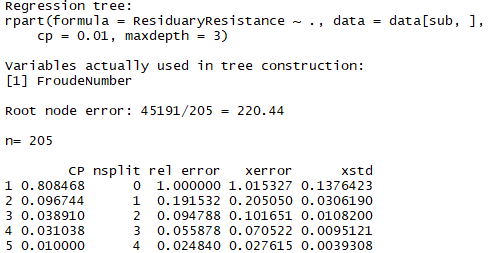
\includegraphics[scale=0.5]{images/pic_38.png}\\

Podemos notar que el valor que corresponde al \textit{xerror} m\'as peque\~no es $cp = 0.01$, el mismo que utilizamos para crear el \'arbol inicial. 

Otra forma de ver el \textit{cp} \'optimo es graficar el conjunto de posibles podas de costo-complejidad de un \'arbol. Para las medias geom\'etricas de los intervalos de valores \textit{cp} para los que una poda es \'optima, se ha realizado una validaci\'on cruzada en la construcci\'on inicial por \textbf{rpart}.\\

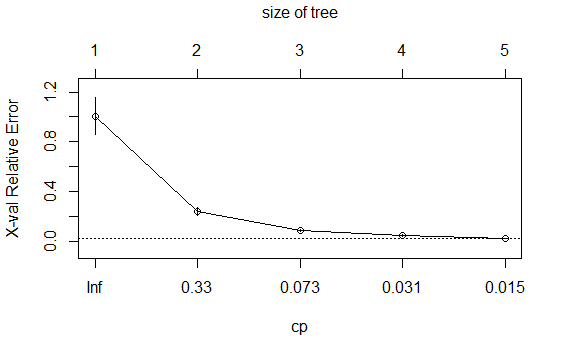
\includegraphics[scale=0.5]{images/pic_39.png}\\

Una buena opci\'on \textit{cp} para podar es a menudo el valor m\'as a la izquierda para el que la media se encuentra por debajo de la l\'inea horizontal. Se puede observar que esto ocurre alrededor del mismo valor de \textit{cp} utilizado.

Ahora bien, necesitamos ser m\'as sistem\'aticos para indagar qu\'e tan bien hace predicciones nuestro modelo. Para ello generamos un vector de predicciones utilizando nuestro conjunto de prueba que contendr\'a los valores predichos por el modelo que hemos entrenado. Posteriormente cruzamos la predicci\'on con los datos reales de nuestro conjunto de prueba para generar una matriz de confusi\'on a partir de la cual se calcular\'a el error.\\

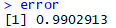
\includegraphics[scale=0.7]{images/pic_40.png}\\

Este valor de error es bastante elevado, lo que quiere decir que nuestro \'arbol no es efectivo.

\subsection{Conclusiones}
A lo largo de este informe se analizaron conjuntos de datos, pudiendo caracterizar su comportamiento gracias a las t\'ecnicas de regresi\'on lineal, ANOVA y reducci\'on de dimensi\'on.

\end{multicols}{2}
\end{document}